% Define document class, paper type and font size.
\documentclass[a4paper,11pt]{report}
% Define font type. Helvetica is the same as Arial.
\usepackage{helvet}
\renewcommand\familydefault{\sfdefault}
% Define margin size.
\usepackage[margin=2cm]{geometry}
% Double spacing.
\usepackage{setspace}
\doublespacing
% Package that allows us to write maths.
\usepackage{amsmath}
% package for more maths symbols
\usepackage{amssymb}
\usepackage{mathtools}
\usepackage{subcaption}
% Package for links
\usepackage{hyperref}
% Package that allows properly formating SI units, and to write standard form.
\usepackage{siunitx}
\sisetup{range-phrase = \text{ -- }}
% Package that allows us to work with graphics.
%\usepackage[dvips]{graphicx}
\usepackage{graphics}
% Package that allows us to use eps files.
\usepackage{epstopdf}
\DeclareGraphicsExtensions{.pdf,.png,.jpg,.eps}
% Package that allows us to import other tex files into this one.
\usepackage{subfiles}
% A bibliography package, and the bibliography file (contained in the same directory as this one).
\usepackage[backend=biber,style=numeric,citestyle=numeric,sorting=none]{biblatex}
\addbibresource{./bibliography.bib}
% Include pdf pages
\usepackage{pdfpages}
% Appendices
\usepackage[titletoc,title]{appendix}
% Tables
\usepackage{tabu}
% Indent first paragraphs
\usepackage{indentfirst}
\usepackage{leading}

% Quote code with highlighting
\usepackage{listings}
% Custom colors
\usepackage{color}
\definecolor{backcolour}{rgb}{0.95,0.95,0.95}
\definecolor{lightgreen}{rgb}{0,0.9,0}
\definecolor{lightorange}{rgb}{1,0.7,0.2}
\definecolor{red}{rgb}{0.9,0,0}
\definecolor{deepgreen}{rgb}{0,0.5,0}
\definecolor{deepblue}{rgb}{0,0,0.5}
\definecolor{deepred}{rgb}{0.5,0,0}
\definecolor{codegray}{rgb}{0.5,0.5,0.5}
% Default fixed font does not support bold face
\usepackage[utf8]{inputenc}
\DeclareFixedFont{\ttb}{T1}{txtt}{bx}{n}{11} % for bold
\DeclareFixedFont{\ttm}{T1}{txtt}{m}{n}{11}  % for normal

\lstdefinestyle{python}{
	language=Python,
	backgroundcolor=\color{backcolour},   
	commentstyle=\color{red},
	otherkeywords={self},             % Add keywords here
	keywordstyle=\color{deepblue},
	numberstyle=\tiny\color{codegray},
	stringstyle=\color{deepgreen},
	basicstyle=\normalsize,
	emph={Mapping}, 		          % Custom highlighting
	emphstyle=\color{deepred},    % Custom highlighting style
	breakatwhitespace=false,         
	breaklines=true,                 
	captionpos=b,                    
	keepspaces=true,                 
	numbers=left,                    
	numbersep=5pt,                  
	showspaces=false,                
	showstringspaces=false,
	showtabs=false,                  
	tabsize=4
}

\lstdefinestyle{C}{
	language=C,
	backgroundcolor=\color{backcolour},   
	commentstyle=\color{red},
	otherkeywords={},             % Add keywords here
	keywordstyle=\color{deepblue},
	numberstyle=\tiny\color{codegray},
	stringstyle=\color{deepgreen},
	basicstyle=\normalsize,
	emph={}, 		          % Custom highlighting
	emphstyle=\color{deepred},    % Custom highlighting style
	breakatwhitespace=false,         
	breaklines=true,                 
	captionpos=b,                    
	keepspaces=true,                 
	numbers=left,                    
	numbersep=5pt,                  
	showspaces=false,                
	showstringspaces=false,
	showtabs=false,                  
	tabsize=4
}

% Keep figures in correct sections
\usepackage{placeins}

\let\Oldsection\section
\renewcommand{\section}{\FloatBarrier\Oldsection}

\let\Oldsubsection\subsection
\renewcommand{\subsection}{\FloatBarrier\Oldsubsection}

\let\Oldsubsubsection\subsubsection
\renewcommand{\subsubsection}{\FloatBarrier\Oldsubsubsection}

% Package to allow images to be on left or right side with text wrapped
\usepackage{wrapfig}
% Number the subsubsections
\setcounter{secnumdepth}{3}

% To do Package (use [disable] to turn off without removing todos)
%\usepackage[colorinlistoftodos]{todonotes}
\usepackage[disable]{todonotes}

% Diagram drawing package -- NOT SURE IF I'LL USE
\usepackage{tikz}
\usetikzlibrary{calc,patterns,decorations.pathmorphing,decorations.markings,shadings,arrows}

% Start document.
\begin{document}
%Title Page
\begin{titlepage}
\begin{center}
\vspace*{1cm}
\Large {\textbf{The University of Oxford}}\\
\Large{\textbf{Engineering Science}}\\
\vfill
\noindent\rule{5in}{0.6pt}\\[1mm]
\huge{\textbf{Fourth Year Project}}\\[3mm]
\Large{\textbf{PiCom: A Digital Communication Test Bed Based on Raspberry Pi}}\\[3mm]
%\todo[inline,color=green!40]{Change/confirm layout of title page -- Must have project title, name, college}
\noindent\rule{5in}{0.6pt}\\[1mm]
\textbf{Candidate}\\
Cameron Eadie\\
Exeter College\\
\textbf{Supervisor}\\
Justin Coon\\
\noindent\rule{5in}{0.6pt}\\[1mm]
\vfill
%\today\\
Trinity Term, 2018\\
\end{center}
\end{titlepage}

% Include Declaration of Authorship
\graphicspath{{./Sections/PDFs/}}
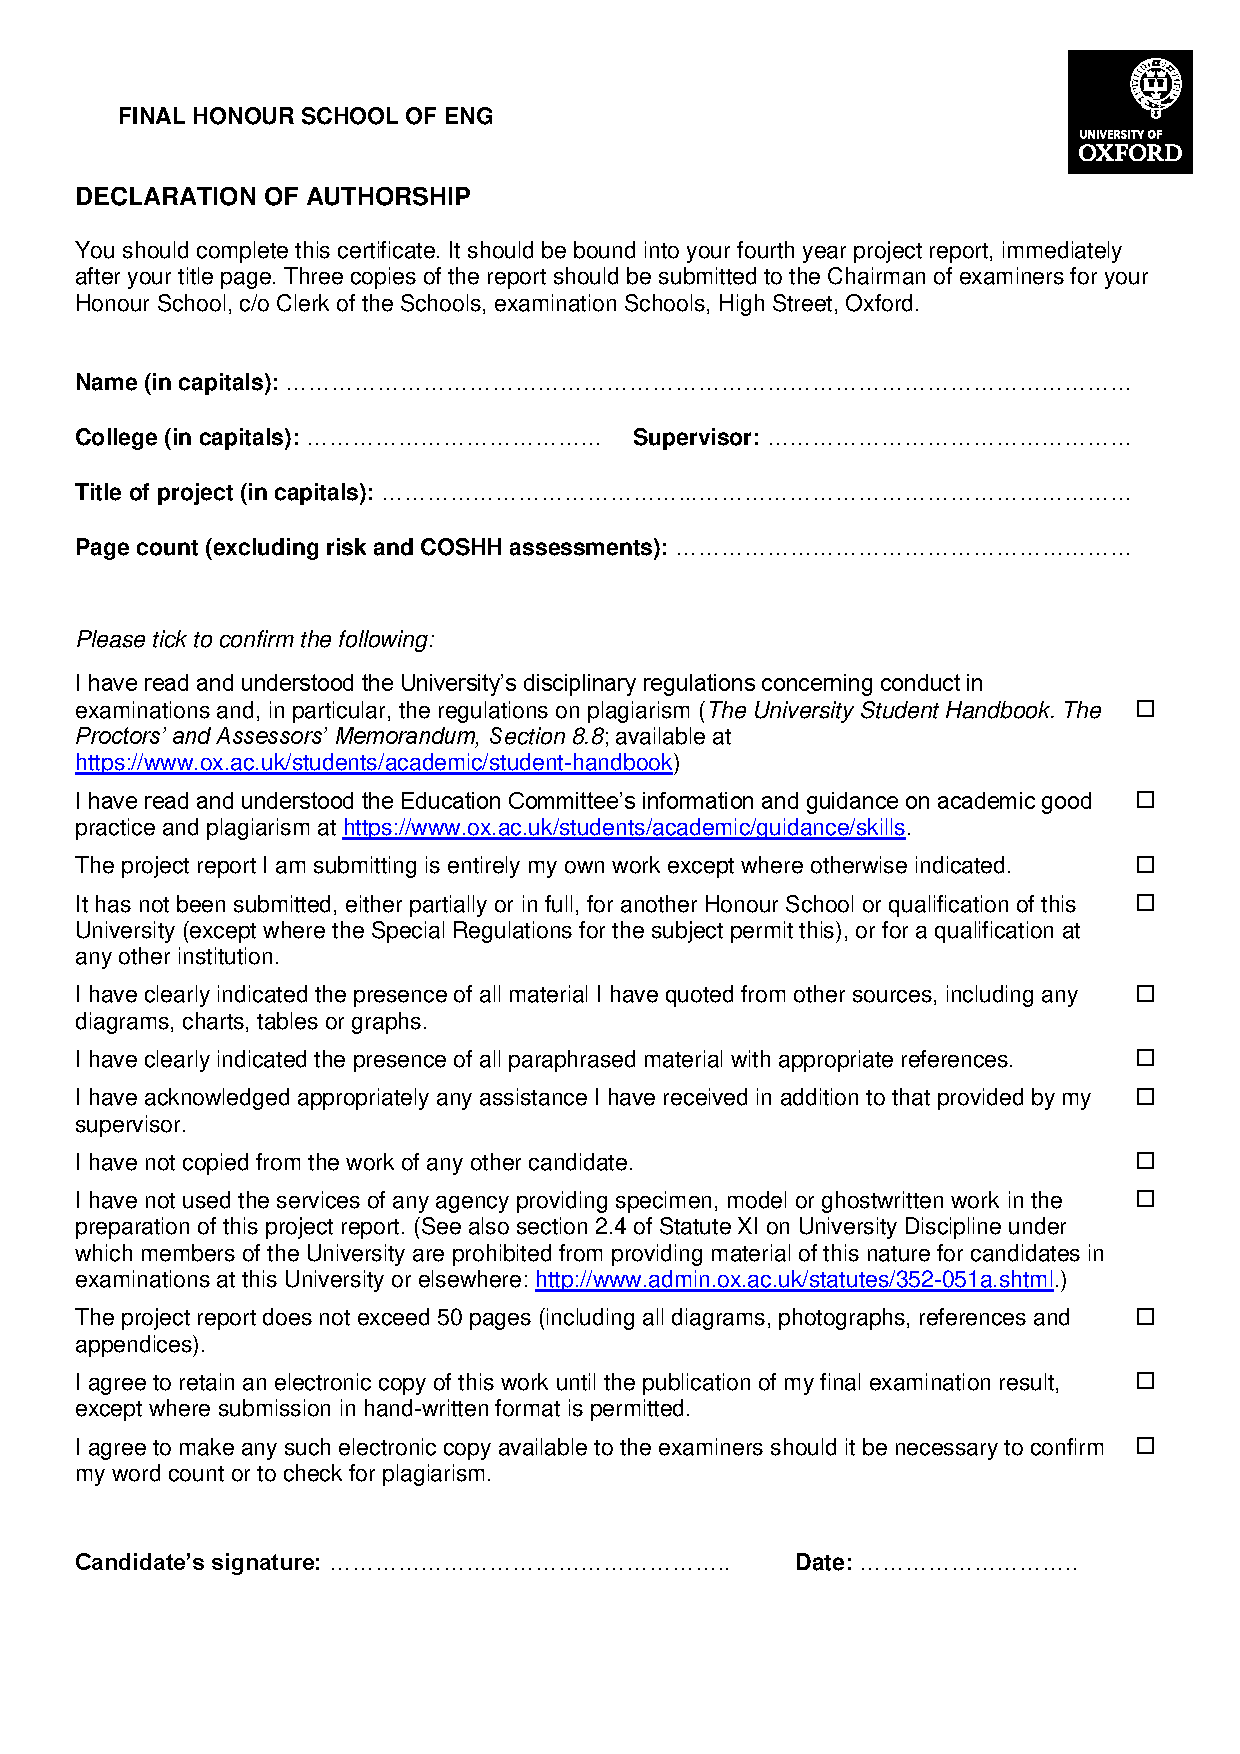
\includepdf[pages={1}]{4YPDeclarationOfAuthorshipForm2018.pdf}

% Abstract
%\textbf{\huge{Abstract}}\\
\begin{abstract}
\subfile{./Sections/Abstract.tex}
\end{abstract}

% Generate the contents page(s).
\pagenumbering{Roman}
\tableofcontents

\listoftodos

% Introduction and Literature Review Chapter.
\chapter{Introduction}
\pagenumbering{arabic}
\setcounter{page}{1}
\graphicspath{{./Sections/Images/}}
\subfile{./Sections/Intro.tex}


% Raspberry Pi Chapter.
\chapter{The Raspberry Pi and the Test Bed} \label{sec_RPi}
\subfile{./Sections/RPi.tex}

% Electronic Testing Chapter.
\chapter{Electronic Testing} \label{sec_Electro Testing}
\subfile{./Sections/Electro_Testing.tex}

% Communications Testing Chapter.
\chapter{Communications Testing} \label{sec_Comms Testing}
\subfile{./Sections/Comms_Testing.tex}

% Summary/Overview, Future Directions Chapter.
\chapter{Conclusion}
\subfile{./Sections/Conclusion.tex}

% Print the bibliography and add it to the table of contents.
\clearpage
\leading{17pt}
\printbibliography[heading=bibintoc]

% Include pages from the Risk Assessments
\clearpage
\pagenumbering{alph}
\begin{appendices}
\graphicspath{{./Sections/PDFs/}}
\addappheadtotoc


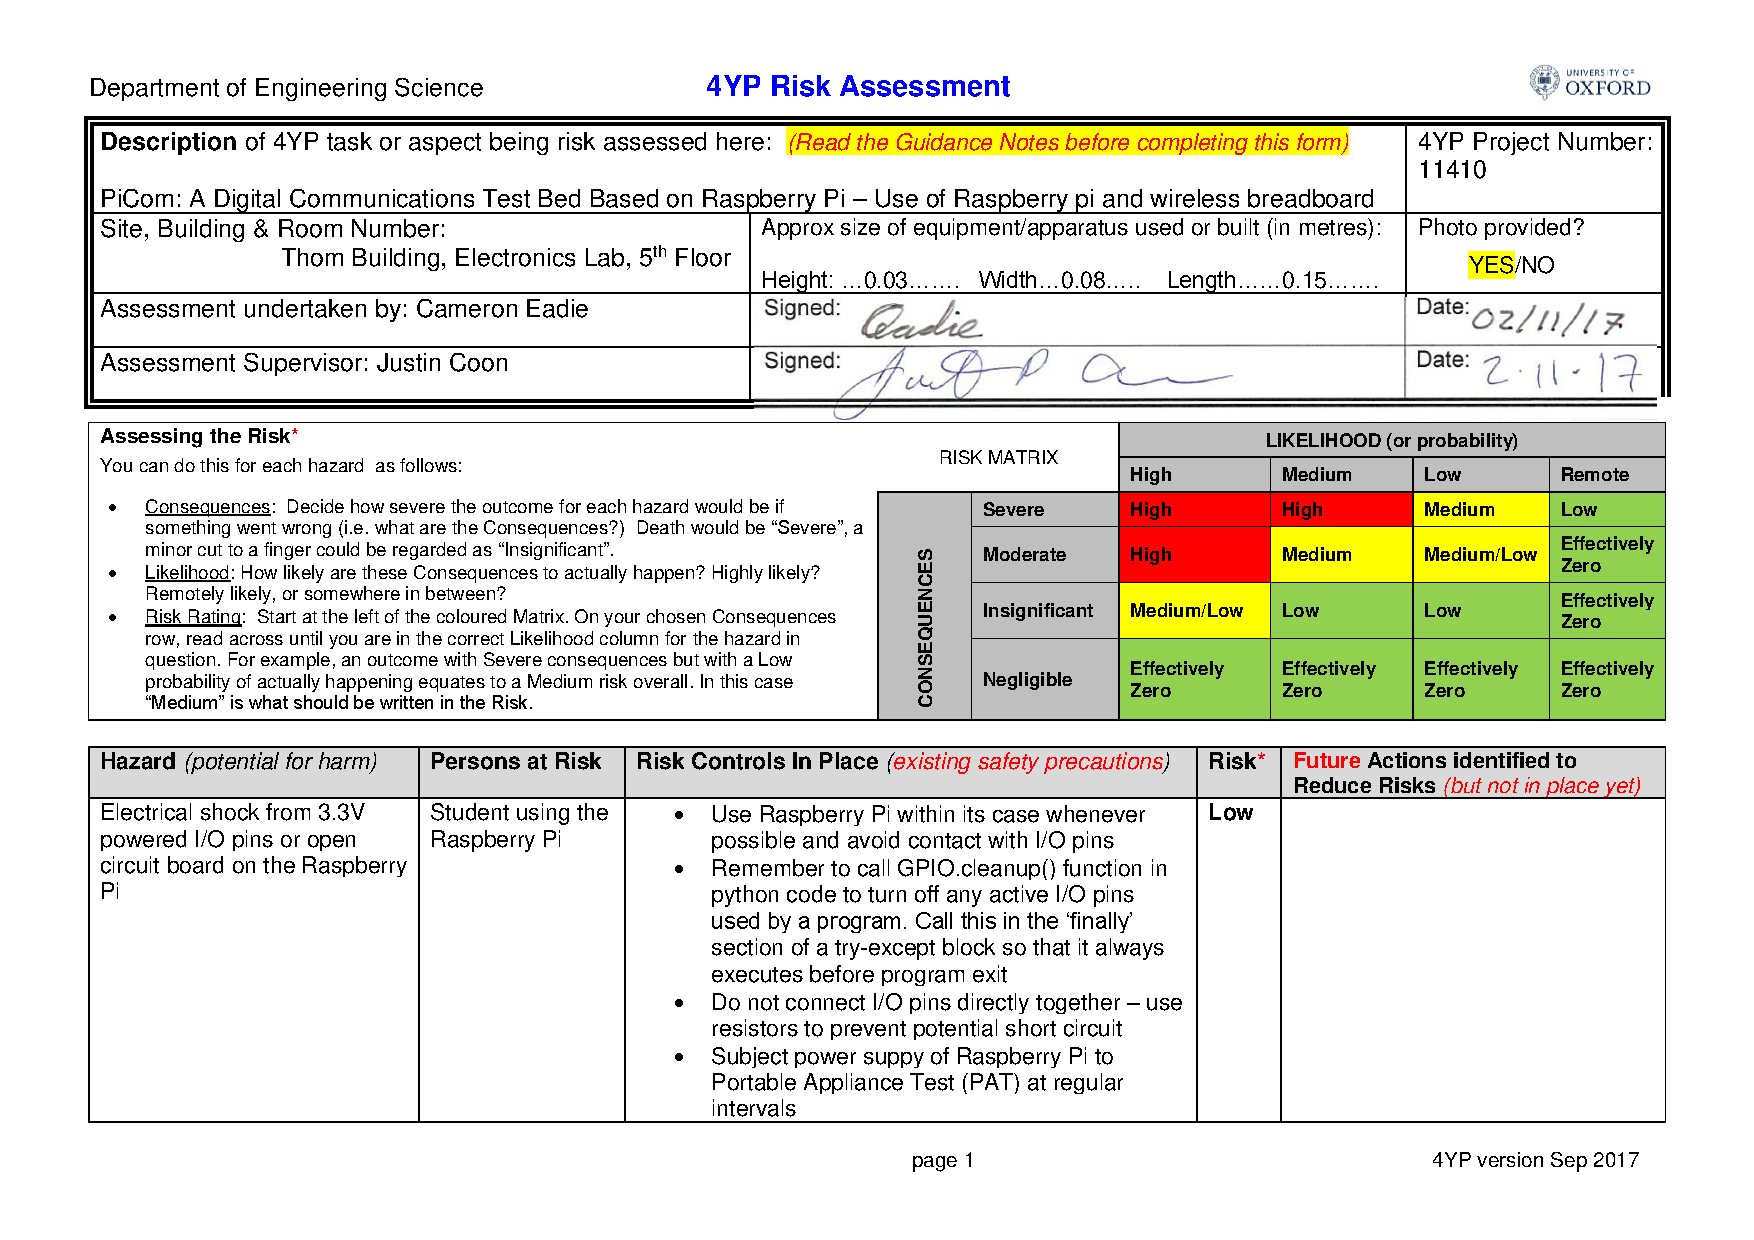
\includepdf[pages=1, pagecommand=\chapter{Risk Assessments}\section{General Risk Assessment}, offset=0 -4cm]{4YPGeneralRiskAssessment.pdf}
\includepdf[pages=2-, pagecommand={}]{4YPGeneralRiskAssessment.pdf}
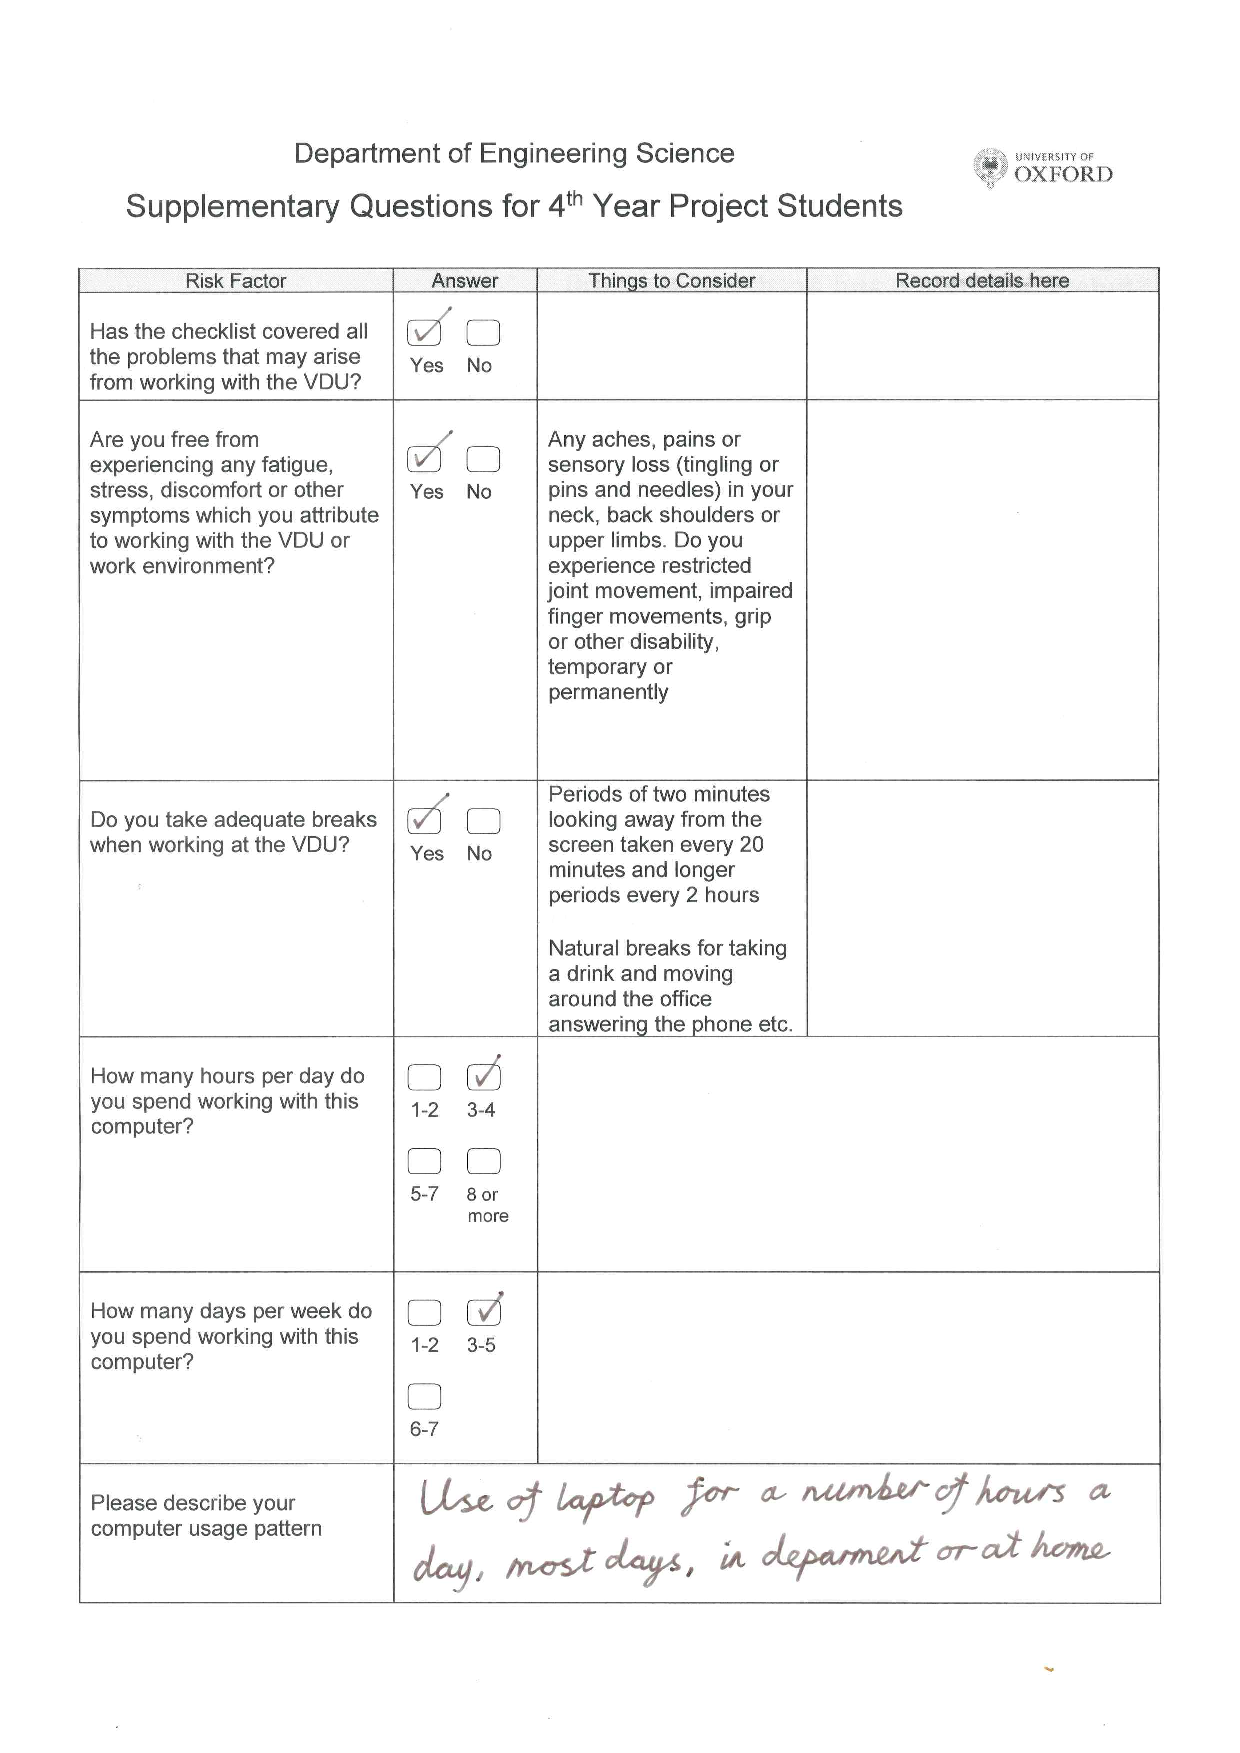
\includepdf[pages=1, pagecommand=\section{Computer Risk Assessment}, offset=0 -1cm]{4YPComputerRiskAssessment.pdf}
\end{appendices}

\end{document}